\iffalse
\documentclass[12pt]{article}
\usepackage{graphicx}
\usepackage[none]{hyphenat}
\usepackage{graphicx}
\usepackage{listings}
\usepackage[english]{babel}
\usepackage{graphicx}
\usepackage{caption} 
\usepackage{booktabs}
\usepackage{array}
\usepackage{amssymb} % for \because
\usepackage{amsmath}   % for having text in math mode
\usepackage{extarrows} % for Row operations arrows
\usepackage{listings}
\usepackage[utf8]{inputenc}
\lstset{
  frame=single,
  breaklines=true
}
\usepackage{hyperref}
  
%Following 2 lines were added to remove the blank page at the beginning
\usepackage{atbegshi}% http://ctan.org/pkg/atbegshi
\AtBeginDocument{\AtBeginShipoutNext{\AtBeginShipoutDiscard}}


%New macro definitions
\newcommand{\mydet}[1]{\ensuremath{\begin{vmatrix}#1\end{vmatrix}}}
\providecommand{\brak}[1]{\ensuremath{\left(#1\right)}}
\newcommand{\solution}{\noindent \textbf{Solution: }}
\newcommand{\myvec}[1]{\ensuremath{\begin{pmatrix}#1\end{pmatrix}}}
\providecommand{\norm}[1]{\left\lVert#1\right\rVert}
\providecommand{\abs}[1]{\left\vert#1\right\vert}
\let\vec\mathbf

\begin{document}

\begin{center}
\title{\textbf{VECTORS}}
\date{\vspace{-5ex}} %Not to print date automatically
\maketitle
\end{center}

\section{10$^{th}$ Maths - EXERCISE-7.4}

Let A(4, 2), B(6, 5) and C(1, 4) be the vertices of $\triangle ABC$
\begin{enumerate}
\item The median from A meets BC at D. Find the coordinates of the point D.
\item Find the coordinates of the point P on AD such that $AP : PD = 2 : 1$
\item Find the coordinates of points Q and R on medians BE and CF respectively such
that $BQ : QE = 2 : 1 \text{and} CR : RF = 2 : 1.$
\item What do yo observe?
\item If $A(x_1, y_1), B(x_2, y_2) \text{and} C(x_3, y_3)$ are the vertices of $\triangle ABC$, find the coordinates of the centroid of the triangle.
\end{enumerate}

Given points are
\begin{align}
\vec{A}=\myvec{4\\ 2} ,
\vec{B}=\myvec{6\\ 5} ,
\vec{C}=\myvec{1\\ 4}
\end{align}
\fi

\begin{enumerate}
\item 
\begin{align}
\vec{D}&=\frac{\vec{B}+\vec{C}}{2}\\
&=\myvec{\frac{7}{2}\\[2pt] \frac{9}{2}}\\
\vec{E}&=\frac{\vec{A}+\vec{C}}{2}\\
&=\myvec{\frac{5}{2}\\ 3}\\
\vec{F}&=\frac{\vec{A}+\vec{B}}{2}\\
&=\myvec{5\\ \frac{7}{2}}
\end{align}

\item 
	For
$n=2$,
\begin{align}
\vec{P}&=\frac{1}{1+n}\brak{\myvec{\vec{A}+n\vec{D}}}\\
&=\frac{1}{3}\myvec{11\\11}
\end{align}

\item 
\begin{align}
\vec{Q}&=\frac{1}{1+n}\brak{\myvec{\vec{B}+n\vec{E}}}\\
&=\frac{1}{3}\myvec{11\\11}\\
\vec{R}&=\frac{1}{1+n}\brak{\myvec{\vec{C}+n\vec{F}}}\\
&=\frac{1}{3}\myvec{11\\11}\\
\end{align}

\item 
 $\vec{P},\vec{Q},\vec{R}$ are the same point.
   
\item 
\begin{align}
\vec{G}&=\frac{\vec{D}+\vec{E}+\vec{F}}{3}\\
&=\frac{1}{3}\myvec{11\\11}\\
\end{align} 
\end{enumerate}
See Fig.  
  \ref{fig:chapters/10/7/4/7/Figure}.
\begin{figure}[h!]
\centering
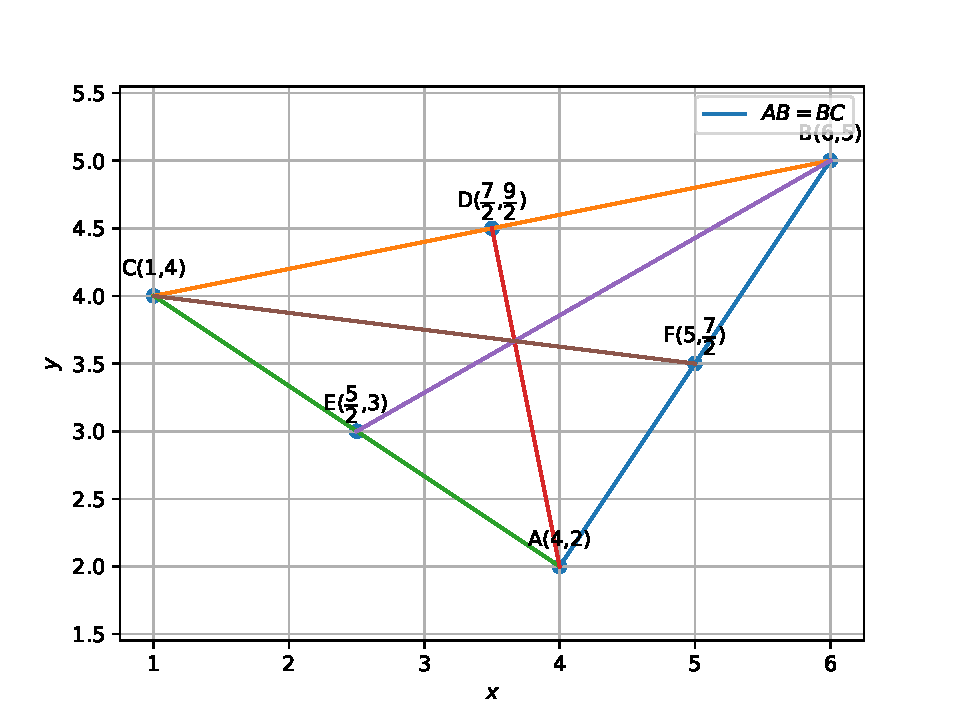
\includegraphics[width=\columnwidth]{chapters/10/7/4/7/figs/dj.pdf}
\caption{}
  \label{fig:chapters/10/7/4/7/Figure}
\end{figure}
